\documentclass[9pt,usenames,dvipsnames]{beamer}

%-------------------------------------------------
%   THEMES & PACKAGES
%-------------------------------------------------
\usetheme[progressbar=frametitle]{metropolis}
\usepackage{graphicx}
\usepackage[export]{adjustbox}
\usepackage{amsmath}
\usepackage{hyperref}
\usepackage{listings}

%-------------------------------------------------
%   COMMON INFO
%-------------------------------------------------
\newcommand{\topicClass}{Software Development Project}
\newcommand{\topicTitle}{Direct Base Controller (DBC)}
\newcommand{\topicDueDate}{23.10.2017}
\newcommand{\presentationShort}{SDP Meeting}
\newcommand{\authorFullName}{Aaqib Parvez Mohammed, Md Zahiduzzaman, Pranjal Dhole, Ramit Sharma} %alphabetical order
\newcommand{\authorGroup}{Group 3}
\newcommand{\authorInstitute}{Hochschule Bonn-Rhein-Sieg}
\graphicspath{{images/}}

%-------------------------------------------------
%   TITLE
%-------------------------------------------------
\title{\topicClass}
\subtitle{\topicTitle}
\date{Presentation date: \topicDueDate}
\author[\authorLastName]{\authorFullName}
\titlegraphic{\hfill
\includegraphics[height=0.7cm]{hbrs_logo.png}}

\setbeamertemplate{footline}[text line]{%
    \parbox{\linewidth}{\vspace*{-8pt}
    \presentationShort\hfill\topicTitle\hfill\authorGroup\hfill\insertpagenumber}}
\setbeamertemplate{navigation symbols}{}

%-------------------------------------------------
%   BEGIN
%-------------------------------------------------
\begin{document}

%-------------------------------------------------
\maketitle

%-------------------------------------------------
\begin{frame}{DBC Code}
	\begin{alertblock}{DBC Components}
	\begin{center}
		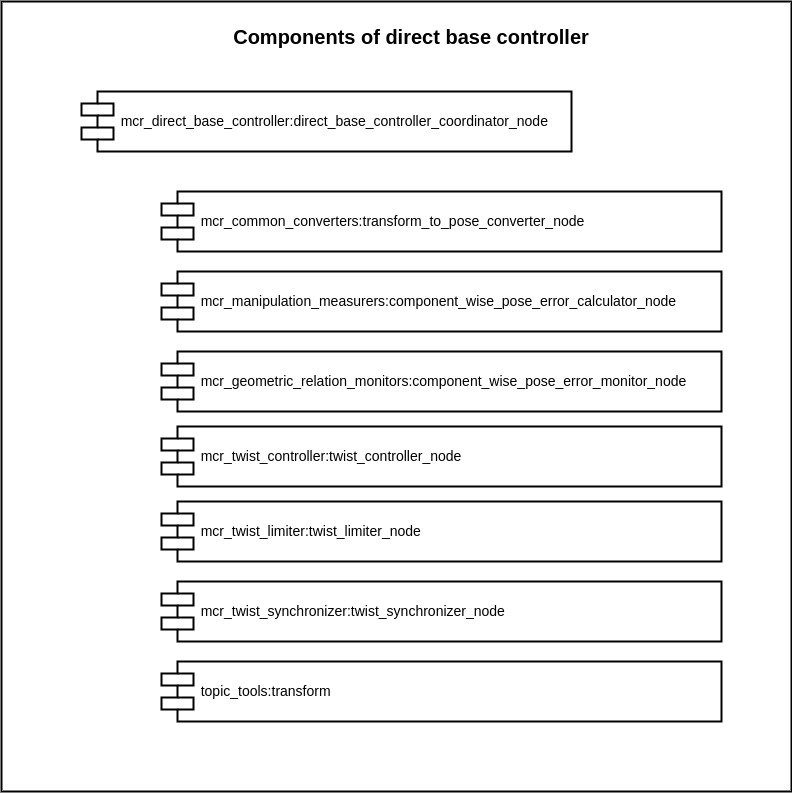
\includegraphics[width=.7\textwidth]{dbc_components.jpeg}
	\end{center}
    \end{alertblock}
\end{frame}

%-------------------------------------------------
\begin{frame}{Tasks}
	\begin{alertblock}{Problem Analysis}
	\begin{itemize}
	\item Merge all nodes into a single node maintaining the modularity of the code.
	\end{itemize}
    \end{alertblock}
    
    \begin{alertblock}{Code Run}
    Working example of project.
    \end{alertblock}
\end{frame}

%-------------------------------------------------
\begin{frame}{DBC project goals}
	\begin{alertblock}{Long term goals}
    	Take all the DBC components and merge them into a single node.
    \end{alertblock}
\end{frame}

%-------------------------------------------------
\begin{frame}{DBC immediate goals}
	\begin{alertblock}{Tasks for next week}
	Understanding component details and their connectivity
    	\begin{itemize}
    	\item {\color{OliveGreen}{Aaqib}}:\\
    	mcr\_direct\_base\_controller:direct\_base\_controller\_coordinator\_node \\
    	mcr\_common\_converters:transform\_to\_pose\_converter\_node
    	\item {\color{OliveGreen}{Pranjal}}:\\
    	mcr\_manipulation\_measurers:component\_wise\_pose\_error\_calculator\_node \\
    	mcr\_geometric\_relation\_monitors:component\_wise\_pose\_error\_monitor\_node
    	\item {\color{OliveGreen}{Ramit}}:\\
    	mcr\_twist\_controller:twist\_controller\_node\\
    	mcr\_twist\_limiter:twist\_limiter\_node
    	\item {\color{OliveGreen}{Zahid}}:\\
    	mcr\_twist\_synchronizer:twist\_synchronizer\_node \\
    	topic\_tools:transform
    	\end{itemize}
    \end{alertblock}
\end{frame}

%-------------------------------------------------
%   END
%-------------------------------------------------
\end{document}
